\section{Experiments}
\label{sec:experiments}

We evaluate DIVI across posterior inference problems that increase in dimension and structure. 
The experiments investigate whether DIVI can capture visible posterior geometry on two-dimensional synthetic targets, approximate a 100-dimensional conditioned diffusion posterior accurately, and provide predictive posterior distributions for Bayesian neural network (BNN) regression.  In line with prior SIVI evaluations, we incorporate annealing techniques where appropriate. 
Unless stated otherwise, tables report the mean and standard error over 10 independent runs.

Our main comparisons are against UIVI and AISIVI \citep{titsias2019unbiased,pielok2025revisiting}.  We also include SIVI \citep{yin2018semi} and KSIVI \citep{cheng2024kernel} where their objectives apply. For the instantiation of the DIVI score model $\psi$, we use a multi-layer perceptron (MLP), which is warm-started before joint training. For each experiment, all methods share the same neural-network architecture for the semi-implicit variational family.
The variational family, evaluation metrics, and per-experiment configurations are collected in Appendix~\ref{app:experiment-details}. We also provide additional arguments to support our theoretical Assumption~\ref{assump:bounded_score} and Assumption~\ref{assump:bounded_reparam} in Appendix~\ref{app: numerical-experiments}.

\subsection{Toy two-dimensional targets}
\label{subsec:toy-experiments}

We first use low-dimensional  unnormalized distribution targets to check whether the learned semi-implicit distribution captures geometric features that are easy to inspect visually.
%ZTW: cited HSIVI explicitly. 
%Done


Following previous works~\citep{yu2023semi,li2023samplingmollifiedinteractionenergy, yu2023hierarchical}, we focus on the three plotted targets in Figure~\ref{fig:toy-scatter-grid}: \texttt{x\_shaped}, \texttt{student\_uc}, and \texttt{8\_gaussians}.  These targets probe for intersecting ridges, heavy-tailed dependence, and multi-modal coverage. We train SIVI, AISIVI, UIVI, and DIVI for 10,000 iterations and KSIVI for 50,000 iterations, with learning rate $10^{-3}$ and batch size 128. For DIVI, we train the proxy score MLP for 5 steps using 2048 samples and learning rate $10^{-3}$ after each update to the main VI model. Full per-method configurations and quantitative diagnostics are given in Appendix~\ref{app:toy-details}.


Figure~\ref{fig:toy-scatter-grid} shows that DIVI preserves the main geometry across the plotted targets, with sample clouds that closely follow the target contours in these visual comparisons.
The quantitative diagnostics in Appendix~\ref{app:toy-details} show that DIVI obtains the lowest mean on four of the six KL-style and Wasserstein metrics and the second-lowest on the remaining two. We also provide a comparison of the learned score against the true target distribution score in Appendix~\ref{app:toy-details}, which demonstrates that DIVI achieves the lowest $L^2$ error on all three targets.

\begin{figure}[t]
  \centering
  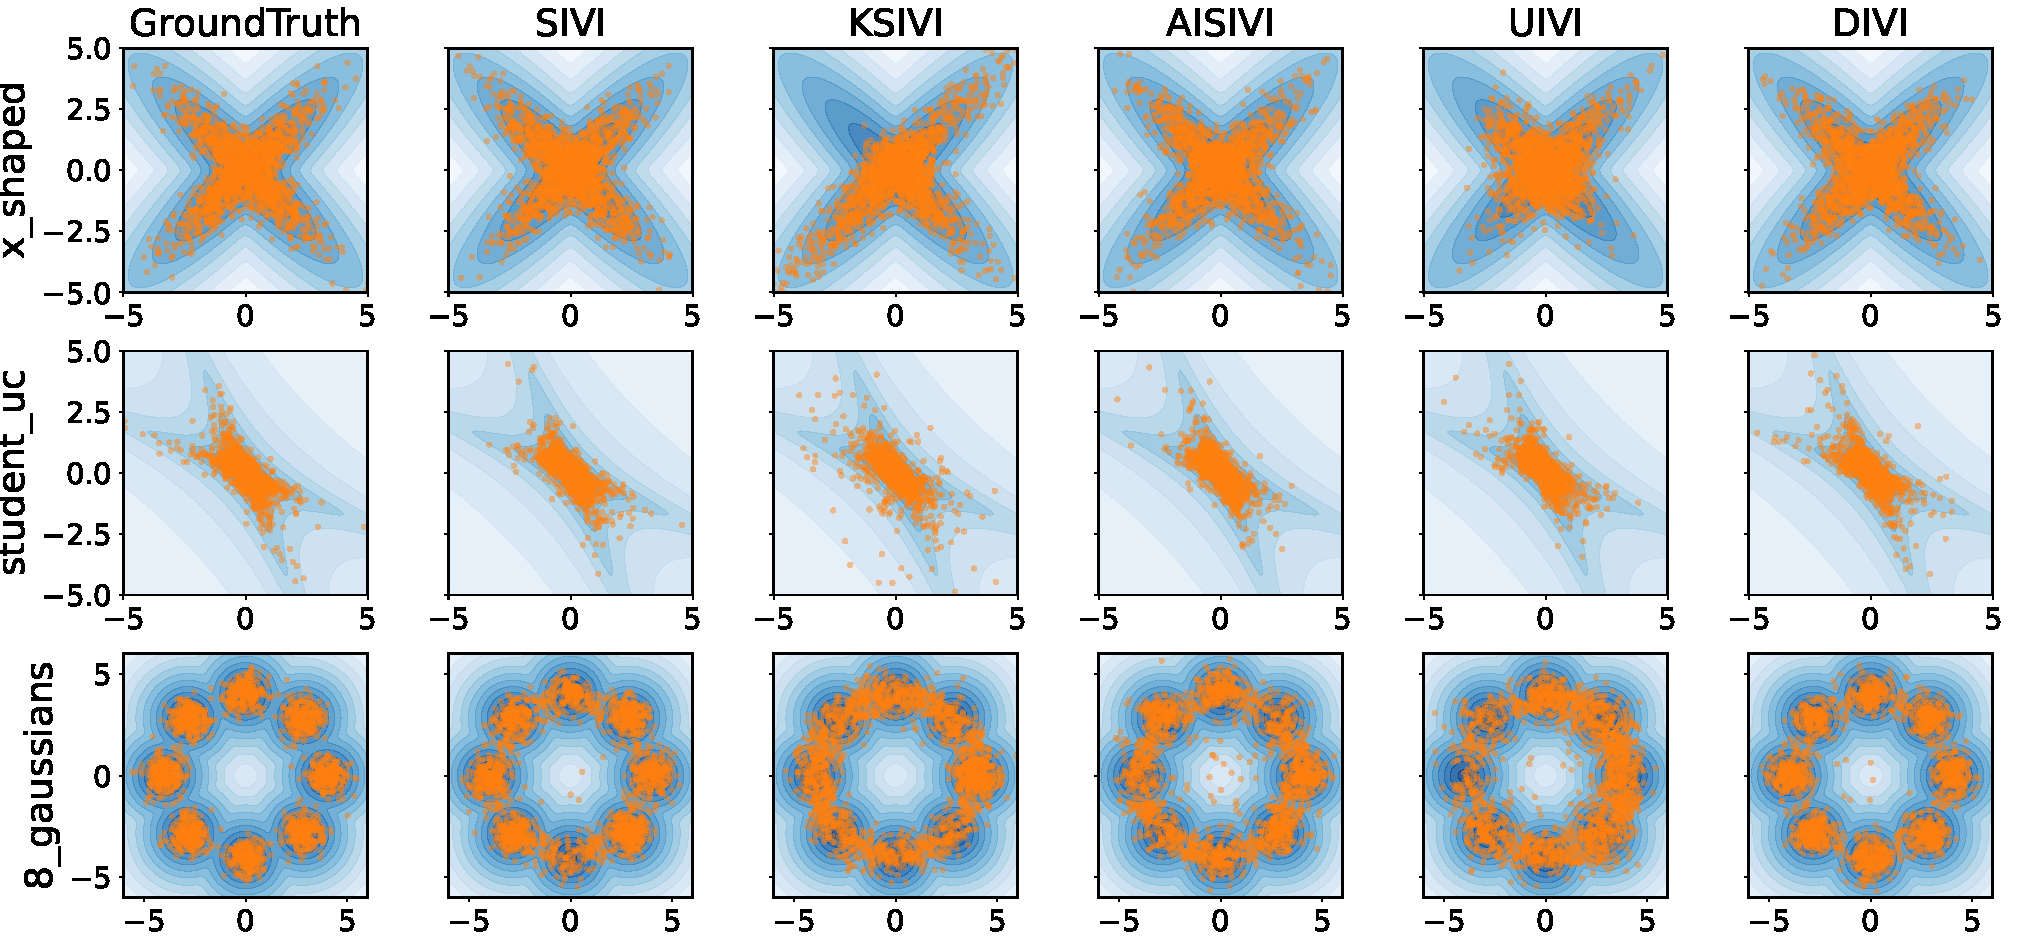
\includegraphics[width=\linewidth]{toy_scatter_grid.pdf}
  \caption{Qualitative comparison on two-dimensional targets.  Each panel is generated from 2,000 samples from the ground-truth baseline or a learned variational distribution; blue contours show the target density.}
  \label{fig:toy-scatter-grid}
\end{figure}

\subsection{Conditioned diffusion process}
\label{subsec:langevin-experiments}

We next evaluate a 100-dimensional conditioned diffusion posterior used in recent SIVI evaluations \citep{cheng2024kernel,pielok2025revisiting}.  The latent path follows the double-well Langevin SDE
\begin{equation}
  dx_t = 10x_t(1 - x_t^2)\,dt + dw_t,
  \qquad 0 \leq t \leq 1,
  \qquad x_0 = 0,
\end{equation}
where $w_t$ is one-dimensional Brownian motion.  We discretize the path with Euler-Maruyama step size $\Delta t=0.01$, giving
$
  x = (x_{\Delta t}, x_{2\Delta t}, \ldots, x_{100\Delta t}) \in \mathbb{R}^{100}.
$
Observations are made every five time steps,
\begin{equation}
  y = (y_{5\Delta t}, y_{10\Delta t}, \ldots, y_{100\Delta t}),
  \qquad
  y_{5k\Delta t} \mid x_{5k\Delta t}
  \sim \mathcal{N}(x_{5k\Delta t}, \sigma^2),
\end{equation}
for $k=1,\ldots,20$ and $\sigma=0.1$.  The inference target is therefore $p(x \mid y) \propto p_{\mathrm{prior}}(x)p(y \mid x)$, with likelihood
\begin{equation}
  p(y \mid x)
  =
  \prod_{k=1}^{20}
  \frac{1}{\sqrt{2\pi\sigma^2}}
  \exp\left\{-\frac{(y_{5k\Delta t}-x_{5k\Delta t})^2}{2\sigma^2}\right\}.
\end{equation}
Posterior quality can be assessed through the mean path and the marginal uncertainty band. Following \citet{cheng2024kernel}, we approximate the posterior by running stochastic gradient Langevin dynamics (SGLD) with 1000 particles, 100,000 iterations and a step size of $10^{-4}$, and use the resulting samples as a high-quality reference for evaluation.
In the evaluation, we include SIVI and KSIVI as additional baselines. We train SIVI, UIVI, AISIVI, and DIVI for 10,000 main VI iterations with learning rate $10^{-3}$ and batch size 128; KSIVI is trained for 100,000 iterations with the same learning rate and batch size and a slower learning rate decay schedule. For DIVI, we train the proxy score MLP for 5 steps using 2048 samples and learning rate $10^{-3}$ after each update to the main VI model. Further method configurations are in Appendix~\ref{app:diffusion-details}.

\begin{figure}[t]
  \centering
  \includegraphics[width=0.9\linewidth]{langevin_trace_grid.png}
  \vspace{-0.2em}
  \caption{Posterior path approximations on the conditioned diffusion benchmark.  The magenta curve is the true latent path, red points are observations, blue curves are posterior mean paths, and shaded regions are marginal 95\% confidence intervals.}
  \label{fig:langevin-trace-grid}
\end{figure}

\input{\finalizationtabledir/langevin_metrics.tex}

Figure~\ref{fig:langevin-trace-grid} shows that DIVI tracks the latent trajectory while maintaining a posterior band comparable to the SGLD reference.  Following \citet{pielok2025revisiting}, Table~\ref{tab:langevin-final-eval} reports the expected log marginal likelihood of the 1,000 high-quality reference samples obtained from SGLD. For each method, we use 100,000 samples from the final trained variational model to approximate the marginal likelihood, and use the marginal likelihood estimated from 100,000 SGLD samples as the reference value. Larger values indicate better agreement with the reference posterior. We also report the wall-clock end-to-end training time for each method, including any warmup phases. As shown in Table~\ref{tab:langevin-final-eval}, DIVI obtains the highest expected log marginal likelihood among the VI methods and is closest to the SGLD reference, while also using the lowest wall-clock training time among the reported variational methods. Further metric and configuration details can be found in Appendix~\ref{app:diffusion-details}.

\subsection{Bayesian neural-network regression}
\label{subsec:bnn-experiments}

We finally evaluate posterior inference for Bayesian neural networks (BNN) on six UCI regression targets: Boston Housing, Concrete, Power Plant, Protein, Wine Red, and Yacht.  Following the BNN settings used for KSIVI and SIVI-SM \citep{cheng2024kernel,yu2023semi}, each target uses a single-hidden-layer ReLU network with 50 hidden units.  These targets provide a diverse high-dimensional suite, with posterior dimensionality ranging from 301 to 751.  Because these posteriors are data-dependent, we evaluate posterior predictive performance through test root mean square error (RMSE) and negative test log-likelihood (NLL), where lower values indicate better performance. We select the learning rate for each method on each target independently from $\{10^{-5}, 10^{-4}, 10^{-3}\}$ via cross-validation. We train all methods for 10,000 VI iterations except KSIVI, which, following the setting in \citet{cheng2024kernel}, is trained for 100,000 iterations. We train the proxy score MLP for DIVI for 2 steps using 2048 samples and learning rate $10^{-3}$ after each optimization step to the variational distribution. Dataset and evaluation details are in Appendix~\ref{app:bnn-details}.

\input{\finalizationtabledir/bnn_rmse_nll.tex}

Table~\ref{tab:bnn-rmse-nll} gives the full predictive comparison across SIVI, UIVI, AISIVI, KSIVI, and DIVI.  DIVI is best or second-best on most reported RMSE and NLL entries, with particularly strong performance on Power and Protein.  The results also show cases where KSIVI remains stronger, such as Wine Red and Yacht RMSE.  Overall, DIVI remains competitive with the strongest baselines while requiring the lowest average wall-clock training time.

\subsection{Ablation studies}
\label{subsec:score-estimation}

First we ablate on the effect of the score estimators of each method. We evaluate SIVI, UIVI, AISIVI, and DIVI as score estimators on the same fixed variational distributions obtained after 2,000 to 10,000 DIVI updates on the X-shaped target. Table~\ref{tab:score-estimation-error} reports the squared $L^2$ discrepancy of the estimated score with respect to a reference score produced by UIVI-styled long HMC chains, together with the score-evaluation time of each method. DIVI achieves the lowest mean score-estimation error at every checkpoint and the lowest score-evaluation latency under the tested configurations. We may also observe that the score estimates of DIVI improves continually throughout the training process. More details of the evaluation are given in Appendix~\ref{app:score-estimation}. We also provide a comparison of the learned score against the true target distribution score along the trajectory of each method in Appendix~\ref{app:toy-details}, which demonstrates that DIVI achieves the lowest $L^2$ error on all three targets.

\begin{table}[!htbp]
\centering
\caption{Score-estimation error on fixed DIVI variational checkpoints for the X-shaped target (mean $\pm$ standard error over five seeds). Bold indicates the lowest mean.}
\label{tab:score-estimation-error}
\small
\setlength{\tabcolsep}{3pt}
\begin{adjustbox}{max width=\linewidth}
\begin{tabular}{lcccc}
\toprule
Checkpoint & SIVI & UIVI & AISIVI & DIVI \\
\midrule
2,000 steps & 154.381 {\footnotesize $\pm$ 68.264} & 1188.717 {\footnotesize $\pm$ 509.566} & 45.529 {\footnotesize $\pm$ 34.394} & \textbf{0.899} {\footnotesize $\boldsymbol{\pm}$ \textbf{0.406}} \\[2pt]
4,000 steps & 113.301 {\footnotesize $\pm$ 27.096} & 889.808 {\footnotesize $\pm$ 239.577} & 13.478 {\footnotesize $\pm$ 8.219} & \textbf{0.802} {\footnotesize $\boldsymbol{\pm}$ \textbf{0.388}} \\[2pt]
6,000 steps & 78.763 {\footnotesize $\pm$ 17.876} & 880.869 {\footnotesize $\pm$ 314.731} & 7.249 {\footnotesize $\pm$ 2.089} & \textbf{0.407} {\footnotesize $\boldsymbol{\pm}$ \textbf{0.211}} \\[2pt]
8,000 steps & 81.909 {\footnotesize $\pm$ 27.307} & 972.443 {\footnotesize $\pm$ 358.567} & 20.203 {\footnotesize $\pm$ 6.899} & \textbf{0.303} {\footnotesize $\boldsymbol{\pm}$ \textbf{0.137}} \\[2pt]
10,000 steps & 107.791 {\footnotesize $\pm$ 21.953} & 899.236 {\footnotesize $\pm$ 273.263} & 6.881 {\footnotesize $\pm$ 3.126} & \textbf{0.331} {\footnotesize $\boldsymbol{\pm}$ \textbf{0.245}} \\[2pt]
\midrule
Time (ms) & 5.316 {\footnotesize $\pm$ 0.082} & 204.523 {\footnotesize $\pm$ 10.375} & 8.096 {\footnotesize $\pm$ 0.099} & \textbf{0.134} {\footnotesize $\boldsymbol{\pm}$ \textbf{0.001}} \\
\bottomrule
\end{tabular}
\end{adjustbox}
\end{table}


Additionally, we ablate on the expressiveness of the semi-implicit variational distributional family, providing comparison with a RealNVP variational family in Appendix~\ref{app:flow-comparison}. We also perform ablations of DIVI's choice of score-update count in each variational optimization step and the reverse batch size in Appendix~\ref{app:reverse-updates}. We believe this would provide practical guidance for future users of DIVI, as the score-update count and reverse batch size are two important hyperparameters in the accuracy-computaion tradeoff of DIVI.
